\subsection{CU13 Eliminar Empleado}
Esta pantalla funciona como un mensaje de seguridad. Al seleccionar un registro de la pantalla 'Visualizar Empleado' y el administrador selecciona la opción de eliminar empleado, se mostrará la siguiente pantalla. Aqui se muestran los datos del empleado que se desea eliminar y dos opciones:
\begin{itemize}
	\item \textbf{Aceptar:} El sistema interactúa con la base de datos y se logra eliminar el registro del empleado. Una vez eliminado, el sistema mostrará un mensaje que el proceso a sido exitoso. (Figura \ref{fig:Alerta Eliminar Empleado - Vista de Escenarios}).
	\item \textbf{Cancelar:} 
\end{itemize}
\begin{figure}[!h]
	\centering
	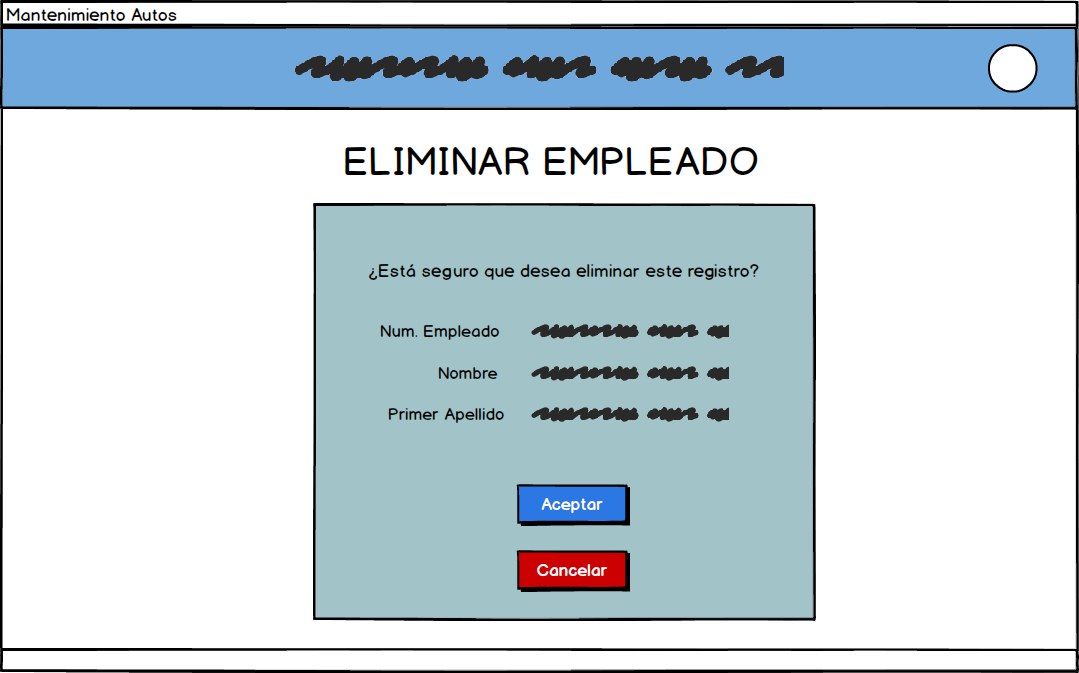
\includegraphics[width=0.8\textwidth]{./diseno/vescenarios/imagenes/eliminarEmpleado}
	\caption{Pantalla Eliminar Empleado - Vista de Escenarios}
	\label{fig:Pantalla Eliminar Empleado - Vista de Escenarios}
\end{figure}
\begin{figure}[!h]
	\centering
	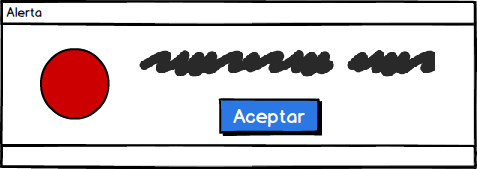
\includegraphics[width=0.5\textwidth]{./diseno/vescenarios/imagenes/alerta}
	\caption{Alerta Eliminar Empleado - Vista de Escenarios}
	\label{fig:Alerta Eliminar Empleado - Vista de Escenarios}
\end{figure}
\clearpage